\section{Introduction}
\label{sec:intro}

\begin{figure}[t]
  \centering
  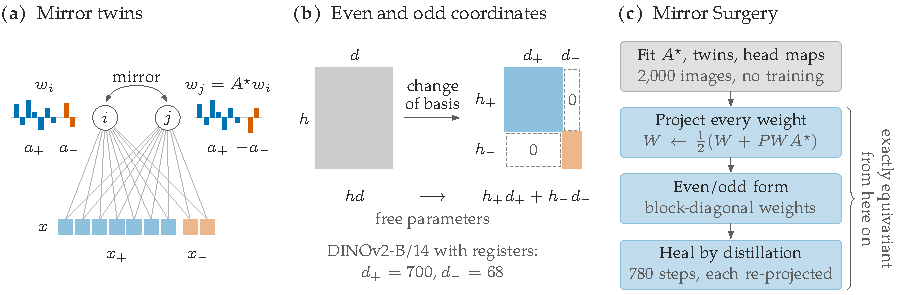
\includegraphics[width=\linewidth]{figures/fig_method.pdf}
  \caption{\textbf{Mirror Surgery.} (a) Twin neurons respond to mirror images of each other, and their input weights are
  related by the stream's mirror operator, $w_j = A^\star w_i$. (b) In the eigenbasis of $A^\star$ an equivariant
  weight matrix is block-diagonal, with an even block and a smaller odd block, so it has
  $h_+ d_+ + h_- d_-$ instead of $hd$ free parameters. (c) The conversion fits the structure from 2{,}000 images, projects
  the weights, rewrites them in even and odd coordinates and heals the model; it is exactly equivariant from the
  projection onwards.}
  \label{fig:method}
\end{figure}

Look inside an early block of a pretrained vision transformer and many of its MLP neurons come in pairs: one neuron
responds to a pattern, and a second neuron responds to the mirror image of that pattern (Figure~\ref{fig:method}a;
real examples in Figure~\ref{fig:twins}).
The network has learned the same feature twice, once for each orientation. This is not surprising for a model trained
with random horizontal flips, which push it to treat an image and its mirror image alike. What is less obvious is how
much of the network the duplication occupies, where it lives, why it is there, and whether it can be turned into a
smaller model.

We call the duplicated part the \emph{symmetry tax}: the share of a layer's weights that would disappear if every twin
pair were stored once. This paper measures the tax, offers a partial explanation of it, and collects it. Our tool is
\emph{Mirror Surgery}, a training-free conversion that rewrites a released vision transformer as a network that is
exactly equivariant to left-right mirroring. In the new basis every feature is either \emph{even} (unchanged when the
image is mirrored) or \emph{odd} (it changes sign), and a pair of twins becomes one even and one odd unit. A short
distillation then recovers the accuracy lost in the conversion (Figure~\ref{fig:method}).

Our contributions are:
\begin{itemize}
  \item \textbf{Where the tax lives} (Section~\ref{sec:structure}). Across 14 released vision models, mirror structure
  is concentrated in the first half of the network, and deep features are almost mirror-invariant. In early blocks the
  structure is about as strong for up-down flips as for left-right flips, much weaker for 90-degree rotations, and of
  similar strength in CLIP and DINOv3, which were trained without flips.
  \item \textbf{Mirror Surgery} (Section~\ref{sec:method}). A conversion of a pretrained ViT into an exactly
  mirror-equivariant network with a flip-invariant class token. In even and odd coordinates the converted DINOv2-B
  with registers has 23.5\% fewer parameters, and the count follows from a standard formula for equivariant linear
  maps.
  \item \textbf{A competitive, exactly invariant model} (Section~\ref{sec:experiments}). After 780 steps of
  distillation, Mirror Surgery matches SVD-LLM, the strongest compressor we tested, at the same size on ImageNet
  $k$-NN (78.34 against 78.06, three seeds each) and on every downstream task we tried. Unlike every compressor, its
  prediction never changes when the image is mirrored (in float32), and it is flip-invariant in one forward pass, 0.66
  points below two-pass flip averaging.
  \item \textbf{What and which way.} In the converted model, the even features recognise bird species as well as the
  full features do but carry essentially no information about which way the bird faces, while the odd features
  predict the facing direction at 99\%.
  \item \textbf{Pre-registration.} We specified the experiments, with pass and fail thresholds, before running them,
  and report all 40 scored predictions, including the 16 that failed (Appendix~\ref{app:prereg}); before healing, for
  example, Mirror Surgery is a weaker compressor than SVD-LLM.
\end{itemize}
